\documentclass{article}
\usepackage{graphicx}

% Prawidłowe dzielenie polskich wyrazów na sylaby przy przenoszeniu do następnej linii
\usepackage[polish]{babel} 

% Aby akceptował polskie litery
\usepackage[utf8]{inputenc}
\usepackage[T1]{fontenc}

% Minimalizacja marginesów
\usepackage[portrait]{geometry}
\geometry{
    left=20mm,
    right=20mm,
    top=20mm,
    bottom=20mm,
    headheight=15pt,
    voffset=10pt,
    footskip=15pt
}

\begin{document}


\section*{0. Projekt 'Rezerwacja kortów tenisowych'}
Cel - Realizacja zadania z baz danych  laboratorium 

\subsection*{1. Opis zawartości}

Baza zawiera dane na temat wynajmów kortów tenisowych pozwalających na wykonanie analiz przychodów dotyczących wynajmu kortów nie zrealizowanych gier na kortach, posiada również informacje o klientach oraz wsparciu kortów pozwalając dokonywać analiz dotyczących ich wynajmu.


\subsection*{2. Ogólny opis domenty}

Wynajem kortów tenisowych buduje problem  związanych z efektywnym i planowym udostępnianiem powierzchni dla zainteresowanych graczy , tworzeniem statystyk wynajmu oraz badaniem jakości obsługi poprzez obserwacje incydentów związanych z utrzymaniem obiektu.
W ramach domeny nie uwzględniamy elementów kosztowych  które leżą w kompetencji działu finansowo księgowego które jako oprogramowanie specjalistyczne  wychodzi poza zakres naszej prostej aplikacji.


\subsection*{3. Możliwe zapytania w języku naturalnym}

\noindent

•	Pokaż raport analizy przychodów dotyczących wynajmu kortów tenisowych dla niezrealizowanych gier na kortach w określonym okresie czasu.\\
•	Udostępnij statystyki wynajmu kortów tenisowych, uwzględniając popularność różnych rodzajów kortów (np. nawierzchnia) oraz godziny największego obłożenia.\\
•	Pokaż raport dotyczący incydentów związanych z utrzymaniem obiektu kortów tenisowych, wraz z danymi na temat rozwiązanych i nierozwiązanych problemów.\\
•	Udostępnij zestawienie danych klientów, którzy korzystali z obsługi kortów tenisowych, wraz z opisem zgłoszonych problemów i ich statusami.\\
•	Pokaż historię rezerwacji danego klienta, wraz z informacjami o zrealizowanych i niezrealizowanych rezerwacjach.\\
•	Udostępnij raporty dotyczące obłożenia kortów w poszczególnych godzinach i dniach tygodnia, aby zoptymalizować planowanie dostępności kortów.\\
•	Pokaż rezerwacje zaplanowane na najbliższy tydzień, wraz z ich statusem.


\subsection*{4. Podstawowe kategorie obiektów i ich atrybuty}

\subsubsection*{Tabela: Korty}
•	KortID (Klucz główny, automatycznie generowany identyfikator)\\
•	NumerKortu (numer identyfikacyjny kortu)\\
•	TypKortu (np. nawierzchnia, oświetlenie)\\
•	CenaGodzinowa (cena za godzinę wynajmu)\\
•	Inne informacje związane z kortem\\

\subsubsection*{Tabela: Klienci}
•	KlientID (Klucz główny, automatycznie generowany identyfikator)\\
•	Imię\\
•	Nazwisko\\
•	Adres\\
•	Telefon\\
•	Email\\
•	Inne informacje o kliencie

\subsubsection*{Tabela: Rezerwacje}
•	RezerwacjaID (Klucz główny, automatycznie generowany identyfikator)\\
•	KortID (Klucz obcy, odniesienie do Kortu)\\
•	KlientID (Klucz obcy, odniesienie do Klienta)\\
•	DataRozpoczęcia (data i godzina rozpoczęcia rezerwacji)\\
•	DataZakończenia (data i godzina zakończenia rezerwacji)\\
•	Opłata (opłata za rezerwację)\\
•	StatusRezerwacji (status rezerwacji, np. Anulowana, Zrealizowana)\\
•	Inne informacje związane z rezerwacją\\

\subsubsection*{Tabela: Pracownicy}
•	PracownikID (Klucz główny, automatycznie generowany identyfikator)\\
•	Imię\\
•	Nazwisko\\
•	Stanowisko\\
•	DataZatrudnienia\\
•	Wynagrodzenie\\
•	Inne informacje o pracowniku

\subsubsection*{Tabela: ObsługaKortow}
•	MaintenanceID (Klucz główny, automatycznie generowany identyfikator)\\
•	KortID (Klucz obcy, odniesienie do Kortu)\\
•	PracownikId (pracownik, odpowiedzialny za realizację zadania)\\
•	DataRaportu (data zgłoszenia konieczności obsługi)\\
•	OpisProblemu (opis problemu, który wymaga obsługi)\\
•	Status (status obsługi, np. w trakcie, zakończona)\\
•	Koszty (koszty związane z obsługą)\\
•	Inne informacje związane z obsługą kortów

\section*{Zestaw zadań nr 2}

\subsection*{Formalne definicje}

Tabela: Korty\\
- KortId (klucz główny, automatycznie generowany identyfikator, np. 1)\\
- NumerKortu (numer identyfikacyjny kortu np Kort1, Kort2)\\
- TypKortu (Możliwości: Otwarty, Zamknięty)\\
- CenaGodzinowa (cena za godzinę wynajmu)\\

Tabela: Klienci\\
- KlientID (Klucz główny, automatycznie generowany identyfikator, np. 1)\\
- Imię (max 50 znaków)\\
- Nazwisko (max 50 znaków)\\
- Adres (max 200 znaków, opcjonalne)\\
- Telefon (max 20 znaków, opcjonalne)\\
- Email (max 50 znaków, opcjonalne)\\

Tabela: Rezerwacje (wszystkie pola wymagane)\\
- RezerwacjaID (Klucz główny, automatycznie generowany identyfikator, np. 1)\\
- KortID (Klucz obcy, odniesienie do Kortu)\\
- KlientID (Klucz obcy, odniesienie do Klienta)\\
- DataRozpoczęcia (data i godzina rozpoczęcia rezerwacji)\\
- DataZakończenia (data i godzina zakończenia rezerwacji)\\
- Opłata (opłata za rezerwację, np 50 PLN)\\
- StatusRezerwacji (Możliwości: Aktywna, Anulowana, Zrealizowana)\\

Tabela: Pracownicy\\
- PracownikID (Klucz główny, automatycznie generowany identyfikator)\\
- Imię (max 50 znaków)\\
- Nazwisko (max 50 znaków)\\
- Stanowisko (max 50 znaków, opcjonalne)\\

Tabela: ObsługaKortow\\
- MaintenanceID (Klucz główny, automatycznie generowany identyfikator)\\
- KortID (Klucz obcy, odniesienie do Kortu)\\
- PracownikId (pracownik, odpowiedzialny za realizację zadania)\\
- DataRaportu (data zgłoszenia konieczności obsługi)\\
- OpisProblemu (opis problemu, który wymaga obsługi)\\
- Status (Możliwe: Zgłoszone, Aktualne, Rozwiazane)\\
- Koszty (koszty związane z obsługą zgłoszenia)\\

\subsection*{Reguły funkcjonowania}

\noindent
REG/001: Dane do systemu wprowadza Operator Kortów\\
REG/002: System ma być dostępny w godzinach 6:00-20:00\\
REG/003: Każdy kort ma unikatową nazwę\\
REG/004: Dane o pracownikach są tylko do odczytu jako pobierane raz dziennie z zewnętrznego system\\
REG/005: Dane o klientach są tylko do odczytu jako pobierane raz dziennie z zewnętrznego system\\

\subsection*{Ograniczenia dziedzinowe}

\noindent
OGR/001: Data rozpoczęcia rezerwacji nie jest datą z przeszłości\\
OGR/002: Data zakończenia  rezerwacji jest nie wcześniejsza niż data rozpoczęcia rezerwacji
OGR/003: CenaGodzinowa nie jest ujemna\\
OGR/004: Email zawiera dokładnie jeden znak '@' s środku\\
OGR/005: Telefon ma format DDD-DDD-DDD, gdzie D reprezentuje pojecyńczą cyfrę

\subsection*{Transakcje}
\subsubsection*{TRA/001}
\textit{Opis:} Edycja kortów\\
\textit{Uwarunkowania:} Zadaniem transakcji jest wyszukiwanie danych o wybranym korcie i edycja tych danych. Edycję wykonuje Operator Kortów\\
\textit{Wejście:} Poprawne dane kortu.\\
\textit{Wyjście:} Dane kortu zapisane w bazie danych\\

\subsubsection*{TRA/002}
\textit{Opis:} Edycja Rezerwacji\\
\textit{Uwarunkowania:} Zadaniem transakcji jest wyszukiwanie danych o wybranej rezerwacji i edycja tych danych. Edycję wykonuje Operator Kortów\\
\textit{Wejście:} Poprawne dane rezerwacji\\
\textit{Wyjście:} Dane rezerwacji zapisane w bazie danych\\

\subsubsection*{TRA/003}
\textit{Opis:} Raportowanie problemów\\
\textit{Uwarunkowania:} Zadaniem transakcji jest wyszukiwanie danych o wybranej rezerwacji i edycja tych danych. Edycję wykonuje dowolny pracownik kortów\\
\textit{Wejście:} Dane o zgłoszonym problemie\\
\textit{Wyjście:} Dane o zgłoszonym problemie\\

\section*{Zestaw zadań nr 3}
\subsection*{Opis zidentyfikowanych encji:}
Korty: Encja ta przechowuje informacje o dostępnych kortach do wynajęcia. Zawiera klucz główny KortID, który jest automatycznie generowanym identyfikatorem. Każdy kort ma przypisany numer identyfikacyjny (NumerKortu), typ (TypKortu - otwarty lub zamknięty) oraz cenę godzinową wynajmu (CenaGodzinowa).\\

\noindent
Klienci: Ta encja zawiera dane klientów korzystających z usług wynajmu kortów. Posiada klucz główny KlientID, który jest automatycznie generowanym identyfikatorem. Informacje o kliencie obejmują imię (Imię), nazwisko (Nazwisko), adres (Adres), numer telefonu (Telefon) i adres e-mail (Email).\\

\noindent
Rezerwacje: Encja ta przechowuje informacje o dokonanych rezerwacjach kortów przez klientów. Posiada klucz główny RezerwacjaID. Każda rezerwacja jest powiązana z konkretnym kortem (KortID) i klientem (KlientID), datą rozpoczęcia (DataRozpoczęcia) i zakończenia (DataZakończenia) rezerwacji, opłatą za rezerwację (Opłata) oraz statusem rezerwacji (StatusRezerwacji).\\

\noindent
Pracownicy: Ta encja zawiera informacje o pracownikach odpowiedzialnych za obsługę kortów. Posiada klucz główny PracownikID. Dane pracowników obejmują imię (Imię), nazwisko (Nazwisko) i stanowisko (Stanowisko).\\

\noindent
ObsługaKortow: Encja ta przechowuje informacje o zgłoszeniach obsługi kortów, takich jak konieczność naprawy lub konserwacji. Posiada klucz główny MaintenanceID. Każde zgłoszenie obsługi kortu jest powiązane z konkretnym kortem (KortID), pracownikiem odpowiedzialnym za realizację zadania (PracownikID), datą zgłoszenia (DataRaportu), opisem problemu (OpisProblemu), statusem zgłoszenia (Status) oraz kosztami związanych z obsługą (Koszty).\\

\subsection*{Klucze encji:}

Korty:\\
Klucz główny: KortID\\

\noindent
Klienci:\\
Klucz główny: KlientID\\

\noindent
Rezerwacje:\\
Klucz główny: RezerwacjaID\\
Klucze obce: KortID (odniesienie do Korty), KlientID (odniesienie do Klienci)\\

\noindent
Pracownicy:\\
Klucz główny: PracownikID\\

\noindent
ObsługaKortow:\\
Klucz główny: MaintenanceID\\
Klucze obce: KortID (odniesienie do Korty), PracownikID (odniesienie do Pracownicy)\\

\subsection*{Związki między encjami}
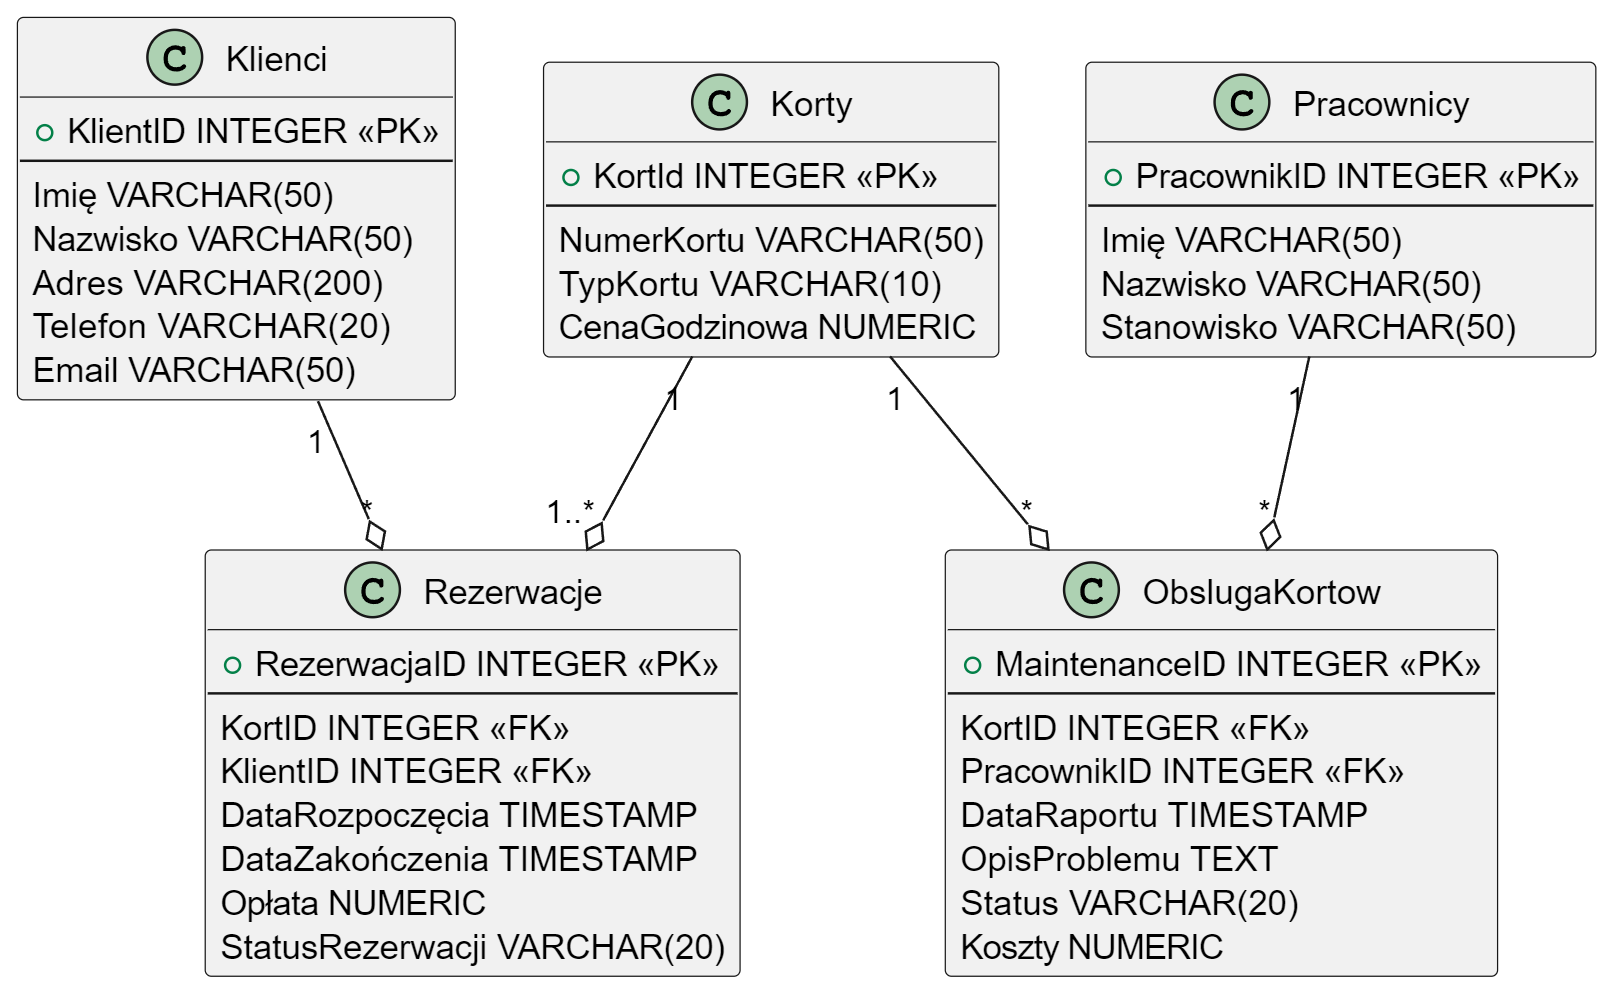
\includegraphics[trim=0 0 0 0,clip,width=\linewidth]{diagram.png}

\subsection*{Związki między encjami}

\noindent
Korty <-> Rezerwacje:\\
Korty mogą być zarezerwowane przez klientów. Jest to relacja wiele do wielu, ponieważ jeden kort może być zarezerwowany przez wielu klientów, a jeden klient może zarezerwować wiele kortów. Relacja ta jest odzwierciedlona przez tabelę pośredniczącą Rezerwacje, która przechowuje informacje o rezerwacjach związanych z konkretnymi kortami.\\

\noindent
Klienci <-> Rezerwacje:\\
Klienci mogą dokonywać rezerwacji kortów. Jest to również relacja wiele do wielu, ponieważ jeden klient może dokonać wielu rezerwacji, a jedna rezerwacja może być dokonana przez jednego klienta. Relacja ta jest odzwierciedlona przez tabelę pośredniczącą Rezerwacje, która przechowuje informacje o rezerwacjach dokonanych przez konkretne osoby.\\

\noindent
Korty <-> ObsługaKortow:\\
Korty mogą wymagać obsługi ze strony pracowników. Jest to relacja jeden do wielu, ponieważ jeden kort może wymagać obsługi, ale wielu pracowników może być odpowiedzialnych za obsługę różnych kortów. Relacja ta jest odzwierciedlona przez tabelę ObsługaKortow, która przechowuje informacje o zgłoszeniach obsługi związanych z konkretnymi kortami.\\

\noindent
Pracownicy <-> ObsługaKortow:\\
Pracownicy są odpowiedzialni za obsługę kortów. Jest to również relacja jeden do wielu, ponieważ jeden pracownik może być odpowiedzialny za obsługę wielu kortów, ale każde zgłoszenie obsługi jest powiązane z jednym pracownikiem. Relacja ta jest odzwierciedlona przez tabelę ObsługaKortow, która przechowuje informacje o przypisanych pracownikach do zgłoszeń obsługi.\\


\subsection*{Diagram zwiazków encji}
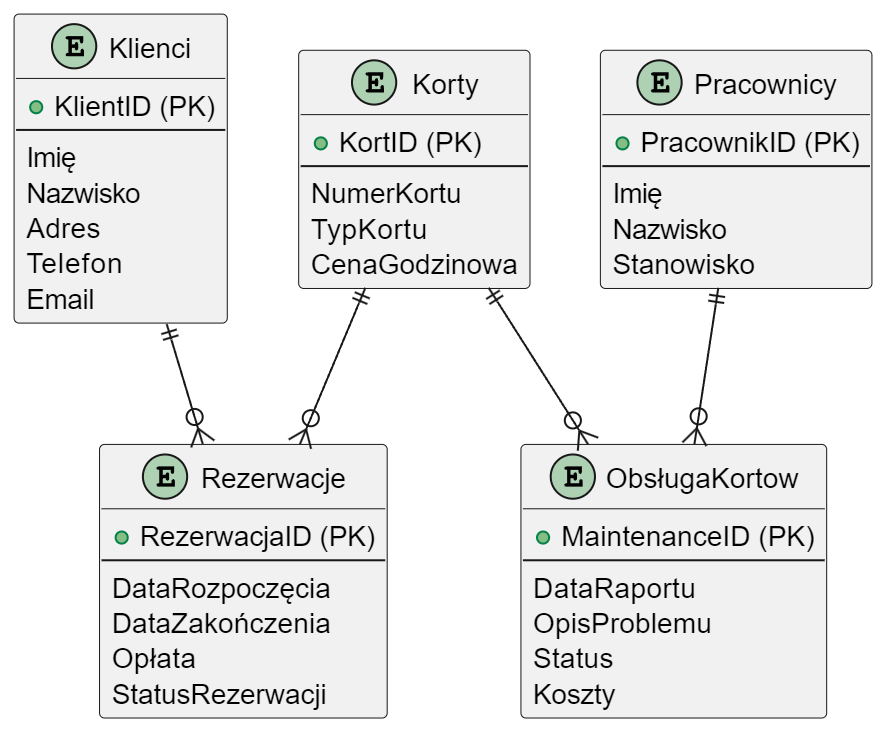
\includegraphics[trim=0 0 0 0,clip,width=\linewidth]{diagram-zwiazkow-encji.png}


\subsection*{Schemat bazy danych}
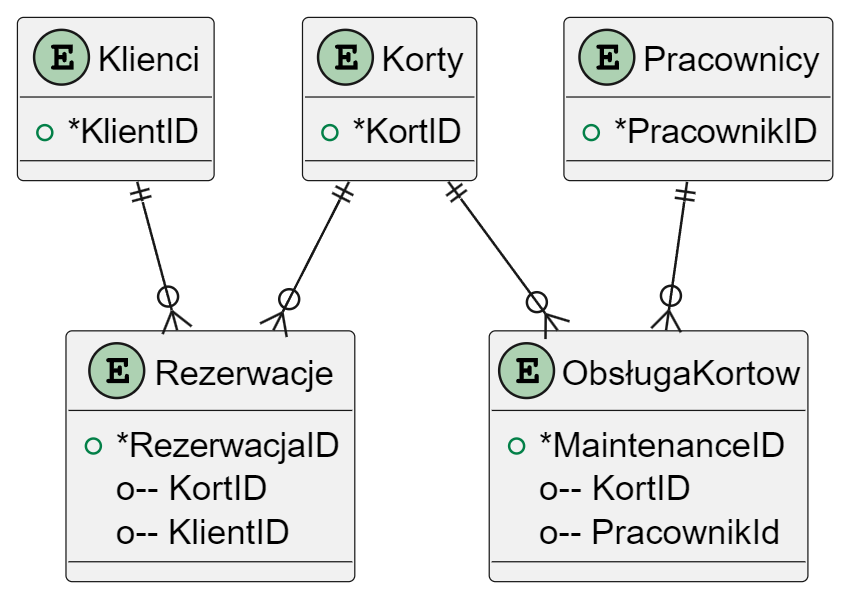
\includegraphics[trim=0 0 0 0,clip,width=\linewidth]{schemat-bazy-danych.png}
\end{document}